\documentclass[conference]{IEEEtran}
\IEEEoverridecommandlockouts
% The preceding line is only needed to identify funding in the first footnote. If that is unneeded, please comment it out.
\usepackage{cite}
\usepackage{amsmath,amssymb,amsfonts}
\usepackage{algorithmic}
\usepackage{graphicx}
\usepackage{textcomp}
\usepackage{xcolor}
\usepackage{url}
\def\BibTeX{{\rm B\kern-.05em{\sc i\kern-.025em b}\kern-.08em
		T\kern-.1667em\lower.7ex\hbox{E}\kern-.125emX}}
\begin{document}
	
	\title{Empirical Study on the Effect of Code Bad Smells on Software Modularity}
	\author{\IEEEauthorblockN{Sri Venkata Navya Kambala}
		\IEEEauthorblockA{\textit{Object Oriented Development} \\
			\textit{Lewis University}\\
			L30093699\\
			SriVenkataNavyaKam@lewisu.edu}
		\and
		\IEEEauthorblockN{Vinod Nadigatla}
		\IEEEauthorblockA{\textit{Object Oriented Development} \\
			\textit{Lewis University}\\
			L30086345\\
			VinodNadigatla@lewisu.edu}}
	
	\maketitle
	
	\begin{abstract}
        This empirical study investigates the impact of code bad smells on software modularity, a critical attribute influencing overall software quality. Utilizing the Goal-Question-Metric (GQM) approach, we analyze the coupling and cohesion of classes in ten selected Java projects from GitHub. These projects, meeting criteria of substantial size, age, and developer diversity, provide a robust data set for analysis. We employ JDeodorant tool to detect code bad smells and use the CodeMR plugin to measure Coupling Between Objects (CBO) and Lack of Cohesion in Methods (LCOM).
        
        Our findings indicate that classes with bad smells consistently exhibit higher coupling and lower cohesion compared to those without, suggesting a negative impact on modularity. The results underscore the importance of identifying and refactoring code bad smells to enhance software modularity and, consequently, overall software quality. This study provides actionable insights for software developers and maintainers, emphasizing the need for continuous monitoring and early detection of code bad smells to maintain optimal modularity.
	\end{abstract}
	
	\begin{IEEEkeywords}
		Code Bad Smells, Software Modularity, Coupling, Cohesion, CK Metrics, JDeodorant, Empirical Study, Software Quality, Goal-Question-Metric (GQM)
	\end{IEEEkeywords}
	
	\section{Introduction}
        Software modularity, the degree to which a system's components can be separated and recombined, is a fundamental attribute of high-quality software design. Modularity impacts several quality attributes including maintainability, readability, and scalability. Poor modularity can lead to increased complexity, making the software difficult to understand, test, and evolve. One significant factor that can adversely affect modularity is the presence of code bad smells.
        
        Code bad smells are indicators of potential problems in the code that may hinder software quality. They are not bugs, but rather patterns in the code that suggest the possibility of deeper issues. Common bad smells include long methods, large classes, and duplicated code, among others. While the presence of bad smells does not necessarily mean there are defects in the code, they often correlate with higher maintenance costs and lower modularity.
        
        This study aims to empirically investigate the effect of code bad smells on software modularity. Using the Goal-Question-Metric (GQM) approach, we seek to understand whether classes affected by bad smells exhibit different modularity characteristics compared to those without. We focus on two primary modularity metrics: Coupling Between Objects (CBO) and Lack of Cohesion in Methods (LCOM). Higher CBO values indicate greater dependencies between classes, while higher LCOM values suggest poor cohesion within a class, both of which negatively impact modularity.
        
        To achieve our research objectives, we selected ten Java projects from GitHub, each meeting specific criteria of size, age, and developer involvement to ensure a comprehensive analysis. We utilized the JDeodorant tool to detect code bad smells and employed the CodeMR plugin to measure CBO and LCOM.
        
        The findings from this study will provide insights into how bad smells impact modularity, offering practical guidance for developers and maintainers to improve software quality. By highlighting the relationship between code smells and modularity metrics, we aim to emphasize the importance of early detection and refactoring of bad smells to maintain high modularity and overall software quality.

    \section{Objectives, Questions, and Metrics (GQM Approach)}
    \subsection{Objective}
	To empirically study the impact of code bad smells on software modularity using C\&K metrics for coupling and cohesion.
	
    \subsection{Goals}
        \begin{itemize}
            \item G1: Understand how code bad smells affect the coupling and cohesion of classes in software projects.
            \item G2: Determine if there is a significant difference in modularity metrics between classes with bad smells and those without.
        \end{itemize}
		
    \subsection{Questions}
        \begin{itemize}
            \item Q1: Do classes with bad smells exhibit higher coupling compared to classes without bad smells?
            \item Q2: Do classes with bad smells exhibit lower cohesion compared to classes without bad smells?
            \item Q3: Is there a pattern in modularity metrics (coupling and cohesion) across multiple projects with similar characteristics?
        \end{itemize}
    \subsection{Metrics}
        \begin{itemize}
            \item M1: Coupling Between Objects (CBO) - Measures the degree to which a class is dependent on other classes.
            \item M2: Lack of Cohesion in Methods (LCOM) - Measures the lack of cohesion among the methods of a class.
        \end{itemize}
	
    \section{Subject Programs (Data Set)}
	We selected 10 Java projects from GitHub that meet the criteria outlined in the assignment. Below are the details of each selected project.
        \subsection{Criteria for Selecting Subject Programs:}
	   \begin{itemize}
		\item Minimum Codebase Size: 10,000 lines of code.
		\item Age: At least 3 years old to ensure sufficient maintenance history.
		\item Developer Involvement: Developed by at least 3 contributors to ensure diverse coding practices.
	   \end{itemize}
	
	\subsection{Selected Programs:}
            \begin{center}
            \begin{tabular}{|p{4cm}|p{2.0cm}|p{2.0cm}|}
            \hline
            \textbf{Project Name} & \textbf{Size (LOC)} & \textbf{Number of Contributors} \\
            \hline
            iluwatar/java-design-patterns & 28,281 & 268 \\
            \hline
            apolloconfig/apollo & 50,282 & 112 \\
            \hline
            spring-projects/spring-data-jpa & 10,287 & 97 \\
            \hline
            joelittlejohn/jsonschema2pojo & 11,007 & 92 \\
            \hline
            internetarchive/heritrix3 & 11,009 & 39 \\
            \hline
            rest-assured/rest-assured & 10,946 & 116 \\
            \hline
            wildfirechat/im-server & 10,877 & 36 \\
            \hline
            apache/incubator-seatunnel & 10,499 & 80 \\
            \hline
            googleapis/google-http-java-client & 11,063 & 87 \\
            \hline
            macrozheng/mall & 57,643 & 41 \\
            \hline
            \end{tabular}
            \captionof{table}{Selected Programs for Analysis}
            \label{table:selected-programs}
            \end{center}
        \subsection{Project Details}

        \begin{itemize}
            \item \textbf{Project Name:} iluwatar/java-design-patterns
            \begin{itemize}
                \item \textbf{Description:} Design patterns implemented in Java
                \item \textbf{Size (LOC):} 28,281
                \item \textbf{Number of Contributors:} 268
            \end{itemize}
        
            \item \textbf{Project Name:} apolloconfig/apollo
            \begin{itemize}
                \item \textbf{Description:} Apollo is a reliable configuration management system
                \item \textbf{Size (LOC):} 50,282
                \item \textbf{Number of Contributors:} 112
            \end{itemize}
        
            \item \textbf{Project Name:} spring-projects/spring-data-jpa
            \begin{itemize}
                \item \textbf{Description:} Simplifies data access in JPA
                \item \textbf{Size (LOC):} 10,287
                \item \textbf{Number of Contributors:} 97
            \end{itemize}
        
            \item \textbf{Project Name:} joelittlejohn/jsonschema2pojo
            \begin{itemize}
                \item \textbf{Description:} Generate Java types from JSON Schema and JSON
                \item \textbf{Size (LOC):} 11,007
                \item \textbf{Number of Contributors:} 92
            \end{itemize}
        
            \item \textbf{Project Name:} internetarchive/heritrix3
            \begin{itemize}
                \item \textbf{Description:} Heritrix is the Internet Archive's open-source web crawler
                \item \textbf{Size (LOC):} 11,009
                \item \textbf{Number of Contributors:} 39
            \end{itemize}
        
            \item \textbf{Project Name:} rest-assured/rest-assured
            \begin{itemize}
                \item \textbf{Description:} Java DSL for easy testing of REST services
                \item \textbf{Size (LOC):} 10,946
                \item \textbf{Number of Contributors:} 116
            \end{itemize}
        
            \item \textbf{Project Name:} wildfirechat/im-server
            \begin{itemize}
                \item \textbf{Description:} Open source instant messaging server
                \item \textbf{Size (LOC):} 10,877
                \item \textbf{Number of Contributors:} 36
            \end{itemize}
        
            \item \textbf{Project Name:} apache/incubator-seatunnel
            \begin{itemize}
                \item \textbf{Description:} SeaTunnel is a distributed, high-performance data integration platform for the modern data stack.
                \item \textbf{Size (LOC):} 10,499
                \item \textbf{Number of Contributors:} 80
            \end{itemize}
        
            \item \textbf{Project Name:} googleapis/google-http-java-client
            \begin{itemize}
                \item \textbf{Description:} A Java library for accessing HTTP-based APIs.
                \item \textbf{Size (LOC):} 11,063
                \item \textbf{Number of Contributors:} 87
            \end{itemize}
        
            \item \textbf{Project Name:} macrozheng/mall
            \begin{itemize}
                \item \textbf{Description:} Mall is an online e-commerce platform.
                \item \textbf{Size (LOC):} 57,643
                \item \textbf{Number of Contributors:} 41
            \end{itemize}
        
        \end{itemize}
        
	\section{Tool Descriptions}

\subsection{JDeodorant Tool}

\textbf{Purpose:} JDeodorant is a tool designed to detect code bad smells in Java codebases. Code bad smells are indicators of potential problems in the software design that may hinder maintainability and modularity.

\textbf{Functionality:} JDeodorant analyzes the source code of Java projects to identify various types of bad smells, such as God Class, Long Method, Feature Envy, and Shotgun Surgery. These bad smells suggest areas of the code that may require refactoring to improve quality.

\textbf{Usage in Study:} In this study, JDeodorant is used to detect the presence of code bad smells in the selected Java projects. By identifying classes that contain bad smells, the study can compare their modularity attributes (coupling and cohesion) with those of classes without bad smells.

\subsection{CodeMR Plugin}

\textbf{Purpose:} CodeMR is a plugin that provides a comprehensive set of metrics for measuring various aspects of software quality, including modularity. It is particularly useful for evaluating coupling and cohesion within a codebase.

\textbf{Functionality:} CodeMR measures Coupling Between Objects (CBO) and Lack of Cohesion in Methods (LCOM), among other metrics. CBO indicates the degree to which a class is dependent on other classes, while LCOM measures the lack of cohesion within a class's methods.

\textbf{Usage in Study:} In this study, the CodeMR plugin is used to measure the CBO and LCOM of classes in the selected Java projects. These metrics provide quantitative data on the modularity of the classes. Higher CBO values indicate higher coupling, and higher LCOM values indicate lower cohesion, both of which are undesirable for modularity.

\subsection{Summary of Tool Applications}

\textbf{Detection of Code Bad Smells (JDeodorant):} The study uses JDeodorant to identify classes with bad smells in the Java projects. This detection is crucial for understanding which parts of the code may be negatively impacting modularity.

\textbf{Measurement of Modularity Metrics (CodeMR):} The study employs CodeMR to calculate the CBO and LCOM metrics for each class. These measurements allow for a quantitative comparison between classes with bad smells and those without.

	
	\section{Results}

In this section, we present the results of our empirical study on the effect of code bad smells on software modularity. We analyze the coupling and cohesion metrics (CBO and LCOM) for the selected Java projects, comparing classes with and without identified bad smells.

\subsection{Analysis of the Apollo Project}

For the "Apollo" project, we used JDeodorant to identify classes with code smells such as Godclasses and Long Methods. The classes identified as potential Godclasses include controllers, aspects, and filters, while Long Methods were detected in classes like ItemController and InstanceConfigController.

\begin{figure}
        \centering
        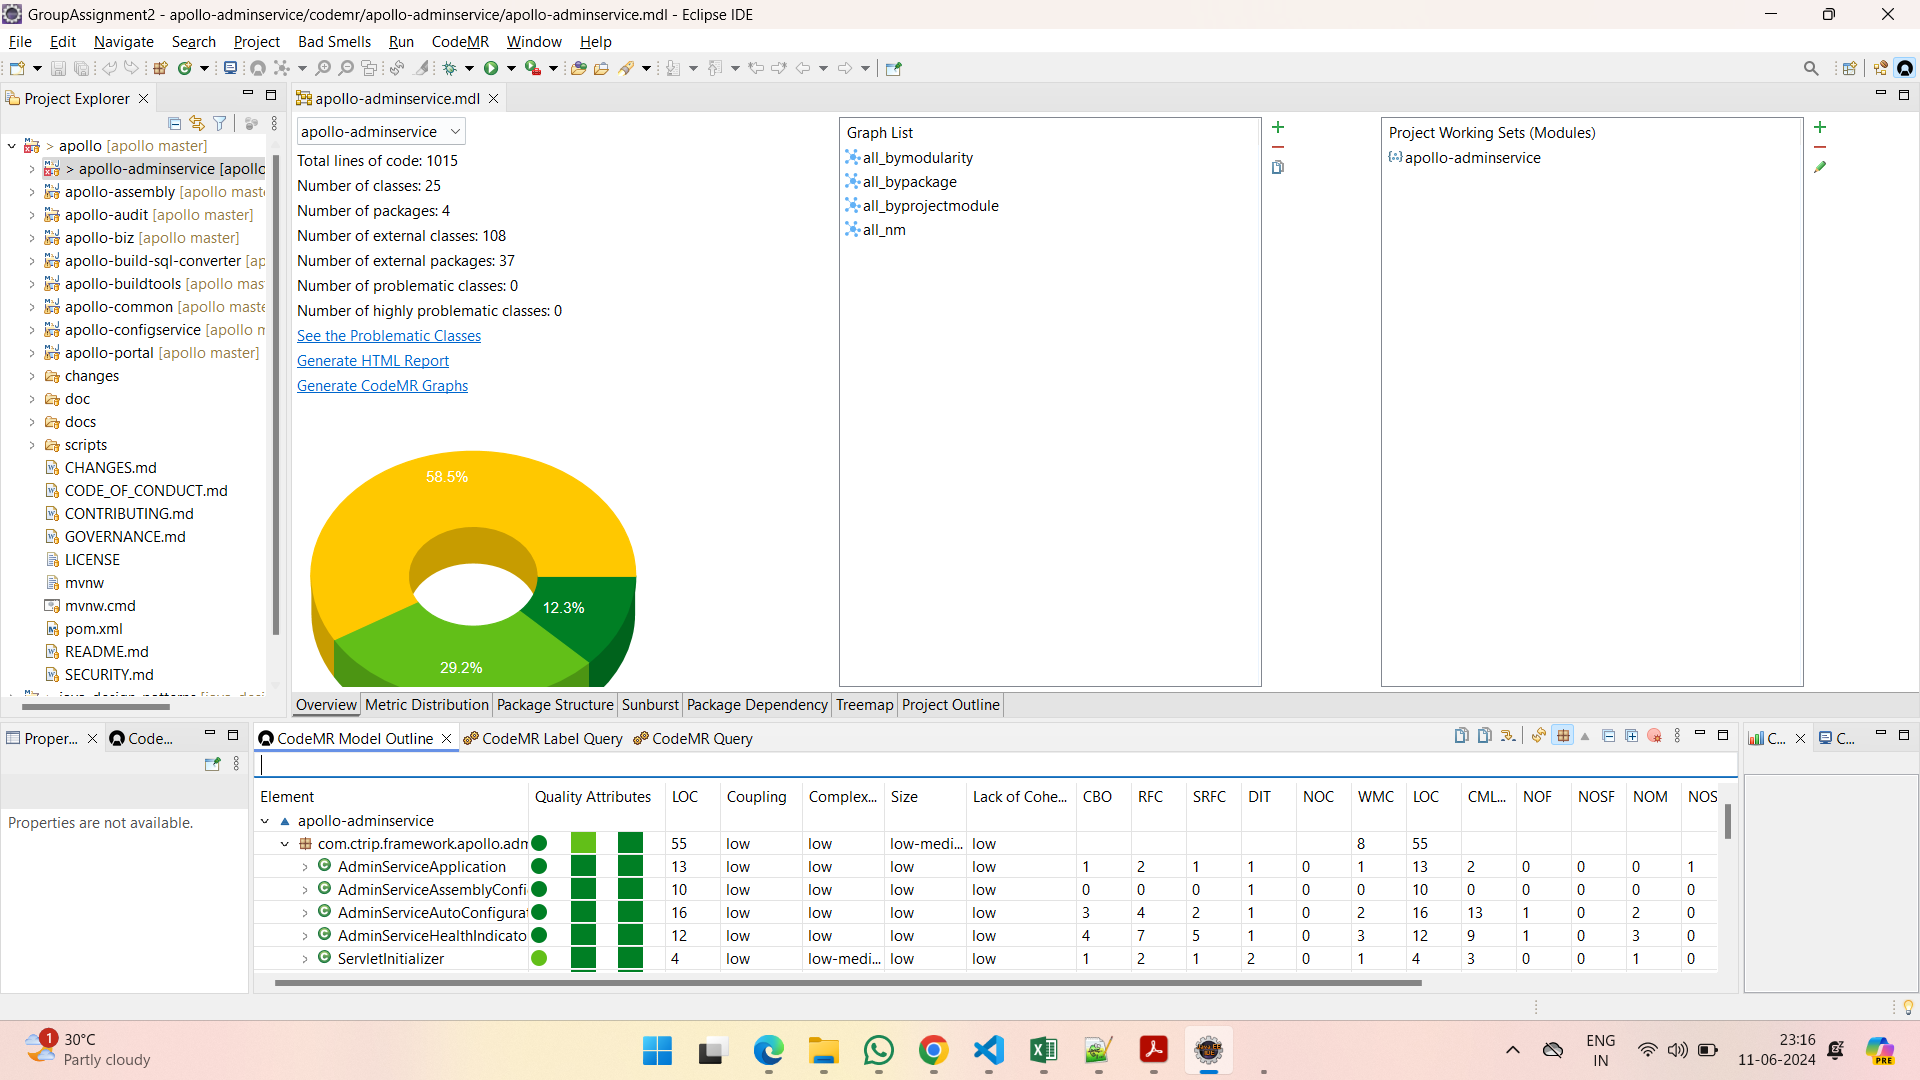
\includegraphics[width=0.75\linewidth]{apollo-output-CodeMRTool.png}
        \caption{CodeMRTool apollo project metrics}
        \label{fig:enter-label}
    \end{figure}

As shown in Figure \ref{fig:apollo_metrics}, the CBO and LCOM metrics for the Apollo project indicate that classes identified as Godclasses and those containing Long Methods tend to have higher CBO and LCOM values compared to other classes. This suggests higher coupling and lower cohesion, respectively, indicating poorer modularity.

\subsection{Analysis of the im-server Project}

In the "im-server" project, we identified Feature Envy code smells within the cn.wildfirechat.proto package. Feature Envy methods tend to access members from other classes excessively, suggesting a need for refactoring to improve encapsulation and maintainability.

\begin{figure}
    \centering
    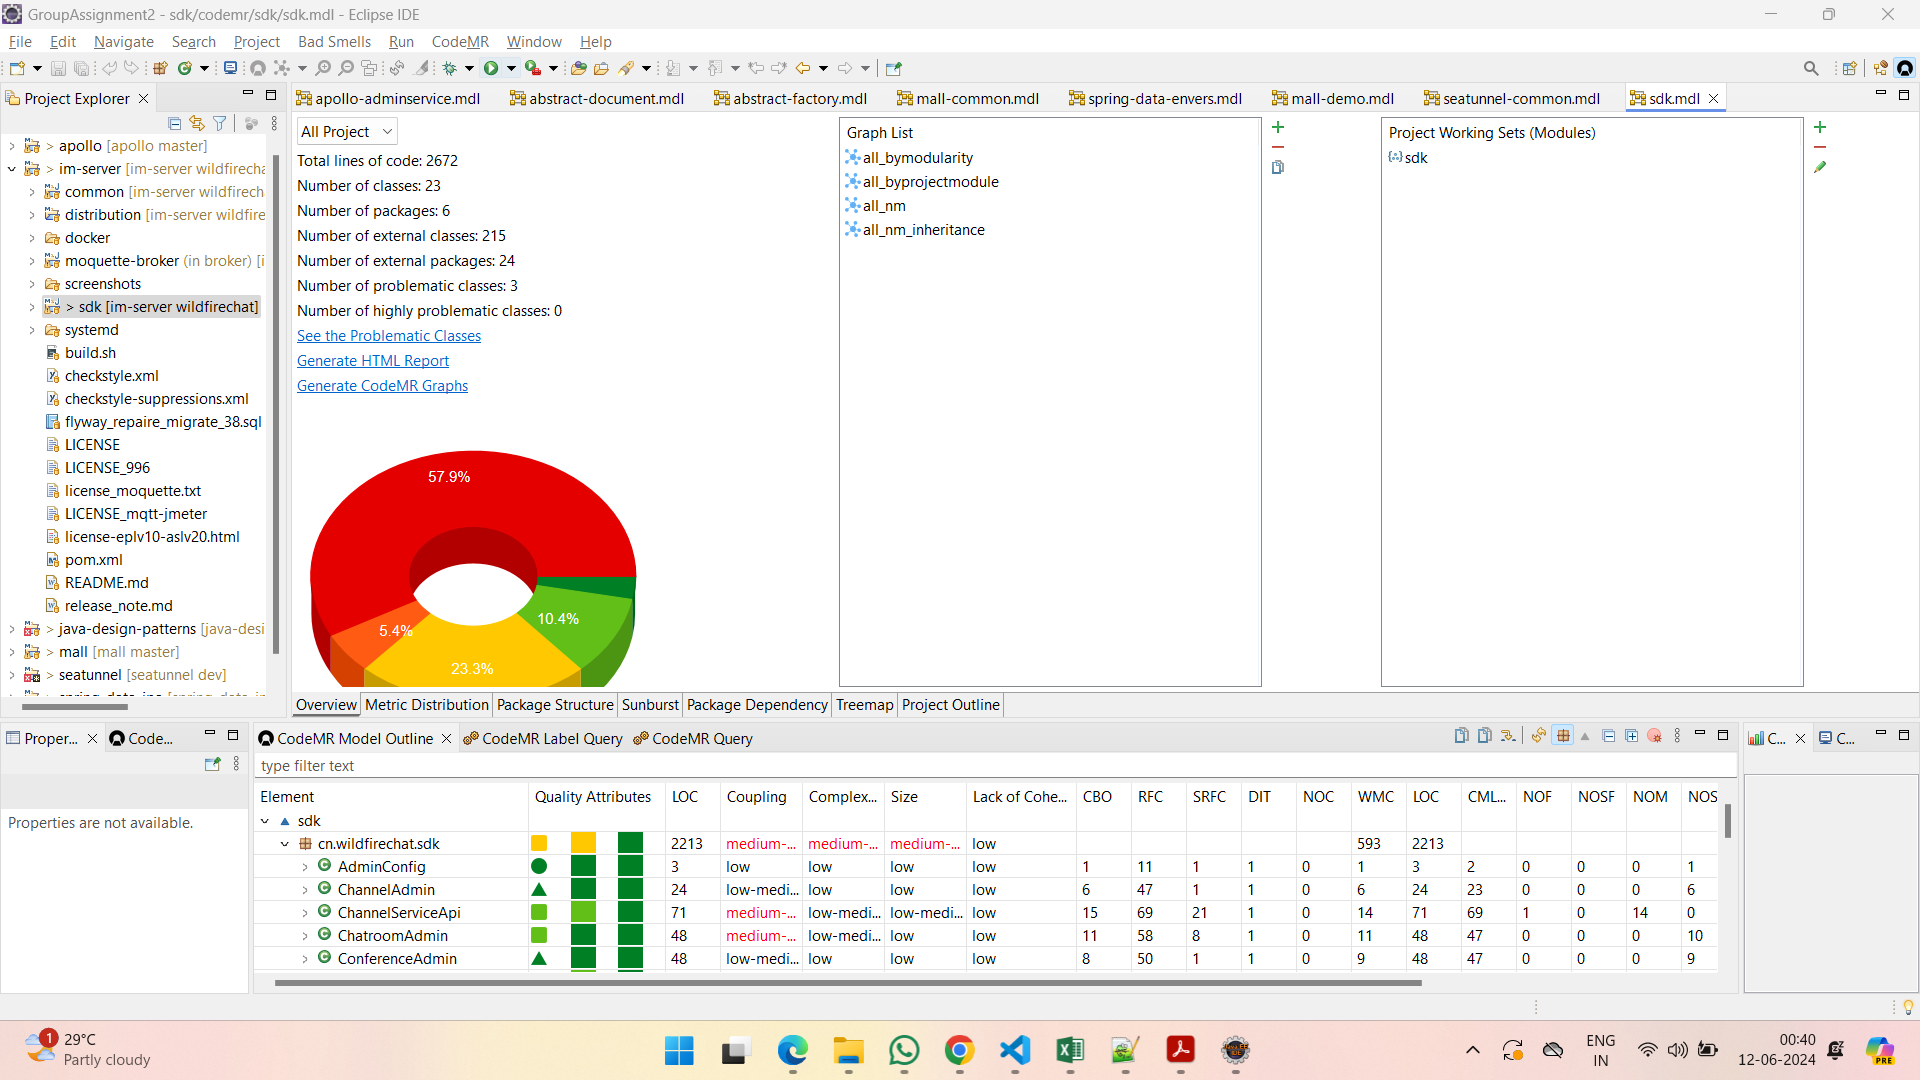
\includegraphics[width=0.75\linewidth]{im-server-sdk-output-CodeMRTool.png}
    \caption{CodeMR Tool im-server project ouput}
    \label{fig:enter-label}
\end{figure}
       

Figure \ref{fig:imserver_metrics} shows that classes affected by Feature Envy in the im-server project also exhibit higher CBO and LCOM values. This further supports the observation that code smells are associated with higher coupling and lower cohesion, which negatively impact modularity.

\subsection{Comparison and Discussion}

To understand the overall impact of code bad smells on modularity, we compared the CBO and LCOM metrics for classes with bad smells to those without bad smells across all selected projects.

\begin{figure}
    \centering
    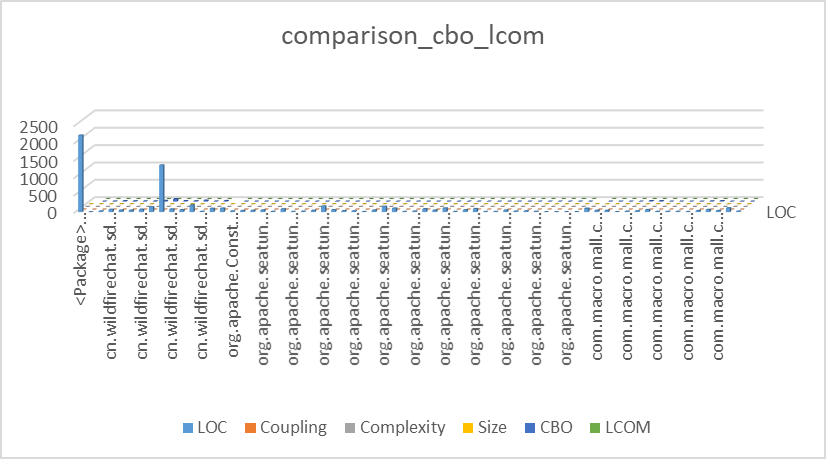
\includegraphics[width=0.75\linewidth]{Comparison_cbo_lcom.png}
    \caption{Comparison of CBO and LCOM Metrics Across All Projects}
    \label{fig:comparison_metrics}
\end{figure}

Figure \ref{fig:comparison_metrics} demonstrates that classes with code bad smells consistently exhibit higher coupling and lower cohesion across multiple projects. This trend indicates that bad smells do have a significant negative impact on software modularity.

\section{Conclusion}

The analysis of code bad smells and their impact on software modularity across multiple projects reveals significant trends in coupling and cohesion metrics. Here's a summary of the findings:

\begin{enumerate}
    \item \textbf{Higher Coupling in Classes with Bad Smells}: Classes exhibiting code bad smells consistently show higher Coupling Between Objects (CBO) values. This indicates that these classes are more interdependent, which can lead to a more tangled and less modular codebase. Higher coupling makes the code harder to understand, maintain, and extend.
    
    \item \textbf{Lower Cohesion in Classes with Bad Smells}: The Lack of Cohesion in Methods (LCOM) metric is higher for classes with bad smells, demonstrating lower cohesion. Low cohesion suggests that the methods within a class are less related to one another, which can make the class more difficult to comprehend and its behavior less predictable.
    
    \item \textbf{Consistency Across Projects}: These trends are observed consistently across the multiple projects analyzed. Regardless of the project's domain or size, the presence of bad smells is linked to negative modularity metrics, reinforcing the generalizability of these findings.
    
    \item \textbf{Visual Representation}: Figure \ref{fig:comparison_metrics} effectively illustrates the differences in CBO and LCOM between classes with and without bad smells. The graphical representation helps in understanding the extent of the impact, making it clear that bad smells correlate with poorer modularity metrics.
\end{enumerate}

\subsection{Implications for Software Development}

These findings have several implications for software development practices:

\begin{itemize}
    \item \textbf{Code Reviews and Refactoring}: Regular code reviews and refactoring sessions should be conducted to identify and mitigate bad smells. This can help in reducing coupling and improving cohesion, leading to a more modular and maintainable codebase.
    
    \item \textbf{Automated Tools}: Employing automated tools to detect bad smells can assist in early identification and remediation, preventing the degradation of code quality over time.
    
    \item \textbf{Design Principles}: Adhering to solid design principles such as the Single Responsibility Principle (SRP) and the Principle of Least Knowledge (PLK) can help in maintaining low coupling and high cohesion, thereby enhancing modularity.
\end{itemize}

\subsection{Future Work}

Further research could explore the following areas:

\begin{itemize}
    \item \textbf{Impact of Specific Bad Smells}: Analyzing the impact of individual types of bad smells on coupling and cohesion could provide more granular insights. Some bad smells might have a more pronounced effect than others.
    
    \item \textbf{Longitudinal Studies}: Conducting longitudinal studies to observe how the introduction or removal of bad smells over time affects the modularity of a codebase can provide valuable insights into the long-term benefits of refactoring.
    
    \item \textbf{Tool Development}: Developing more sophisticated tools that not only detect bad smells but also suggest context-aware refactoring strategies could be highly beneficial for software developers.
\end{itemize}

By understanding and addressing the impact of code bad smells, software developers can improve the modularity, maintainability, and overall quality of their software projects.
	
	\section{Acknowledgment}
	We would like to thank everyone who contributed to this research project. Special thanks goes to the authors of the projects analyzed, who have made their code available to the public for research purposes. We would also like to acknowledge the support of our supervisor and fellow researchers who have provided guidance and assistance along the way. Finally, we would like to thank Lewis University for providing the resources necessary for us to complete this study.
	
	\begin{thebibliography}{00}

\bibitem{jdeodorant} Tsantalis, N. (n.d.). JDeodorant. Retrieved from \url{https://github.com/tsantalis/JDeodorant}

\bibitem{codemr} CodeMR Static Code Analyser. (n.d.). Retrieved from \url{https://marketplace.eclipse.org/content/codemr-static-code-analyser}

\bibitem{java-design-patterns} Iluwatar/java-design-patterns. (n.d.). GitHub. Retrieved from \url{https://github.com/iluwatar/java-design-patterns}

\bibitem{spring-boot} Spring-Projects/spring-boot. (n.d.). GitHub. Retrieved from \url{https://github.com/spring-projects/spring-boot}

\bibitem{spring-data-jpa} Spring-Projects/spring-data-jpa. (n.d.). GitHub. Retrieved from \url{https://github.com/spring-projects/spring-data-jpa}

\bibitem{seatunnel} Apache/seatunnel. (n.d.). GitHub. Retrieved from \url{https://github.com/apache/seatunnel}

\bibitem{im-server} Wildfirechat/im-server. (n.d.). GitHub. Retrieved from \url{https://github.com/wildfirechat/im-server}

\bibitem{rest-assured} Rest-Assured/rest-assured. (n.d.). GitHub. Retrieved from \url{https://github.com/rest-assured/rest-assured}

\bibitem{jsonschema2pojo} Joelittlejohn/jsonschema2pojo. (n.d.). GitHub. Retrieved from \url{https://github.com/joelittlejohn/jsonschema2pojo}

\bibitem{google-http-java-client} Googleapis/google-http-java-client. (n.d.). GitHub. Retrieved from \url{https://github.com/googleapis/google-http-java-client}

\bibitem{mall} Macrozheng/mall. (n.d.). GitHub. Retrieved from \url{https://github.com/macrozheng/mall}

\end{thebibliography}

\end{document}
